\begin{surferPage}[Chmutov-Octic]{משטח מהמעלה השמינית של צ'מוטוב}
    אחד המאפיינים המעניינים של משטח צ'מוטוב $\text{Chm}_{d}, \ d=8,$
    הוא הסימטריה שלו.
    נוכל לראות זאת גם אם נביט במשוואה:
    \[\text{Chm}_{d}\colon T_d(x) + T_d(y) + T_d(z) + 1 = 0,\]
     כאשר $T_d$ הוא מה שקרוי הפולינום של צֶ'בּישֶב (התמונה משמאל).
    העקומה $T_8(x)+T_8(y)=0$ מוצגת מימין:
    
     \begin{center}
      \begin{tabular}{c@{\quad}c}
        \begin{tabular}{c}
          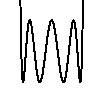
\includegraphics[height=1.75cm]{./../../common/images/Tcheb_008.pdf}
        \end{tabular}    
        &
        \begin{tabular}{c}
          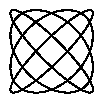
\includegraphics[height=1.75cm]{./../../common/images/Tcheb_2d_008.pdf}
        \end{tabular}    
      \end{tabular}
    \end{center}
    \vspace{-0,3cm}
    המעבר מתמונות אלה לצורת המשטח בתצוגה
    האינטראקטיבית נעשה בשלבים ספורים בלבד.


המשוואות הוצגו על-ידי ס. ו.\ צ'מוטוב בשנות ה-80 המוקדמות.
    באותו זמן, הן היוו שיא עולם של מספר ה-$d$ הגבוה ביותר עבור $\mu(d)$.
    במהלך שנות ה-90, שיפר צ'מוטוב את שיאו האישי, ובשנת 2005 שינו ס. ברסקה,
    א. לאבס וד. ואן-סטראטן (Breske, Labs, van-Straten) את המבנה כדי לקבל משטחים
    ממשיים הכוללים אך ורק נקודות סינגולריות ממשיות.
\end{surferPage}
